\chapter{散乱、双対性、ヴェネツィアーノ振幅}

\lectureoverview{散乱は衝突を実験と比較できる不変なデータに還元する。4つの同一粒子の場合、それらのデータはマンデルスタム変数\(s,t,u\)に整理でき、そのうち独立なのは2つだけである。すると通常の粒子交換は、直接チャネルと交差チャネルを別々に示唆する。ヴェネツィアーノ振幅はその予想を覆した。1つの関数が両方のチャネルの記述を含むのである。講義の後半では、2つの開弦が結合し、1つの振動する鎖として発展し、再び分裂することでその関数を構成する。}

\section{理論が予言すべきもの}

フェルミオン弦は純粋にボソン的な模型の2つの欠陥を解決する。すなわちフェルミオン状態を許容し、適切な射影の後でタキオンを除去する。その臨界時空次元は26ではなく10である。したがって余剰次元は残るが、そのコンパクト化は後回しにされる。当面の主題は散乱である。
\editorialnote{タキオンがないという記述は、必要な射影の後の整合的な超弦スペクトルを指す。世界面フェルミオンを単に加えるだけではそれ自体では十分でない。}

散乱は必ずしも粒子が行う最も興味深い事象ではない。それは単に、実験がきれいに繰り返すことのできる操作である。指定した粒子を互いに向かって送り出し、衝突から現れる粒子を記録し、相互作用領域の内部に隠された力学を推論する。理論は、複素振幅
\begin{equation}
  \mathcal A(\hbox{incoming data}\to\hbox{outgoing data}),
\end{equation}
を与えるとき定量的になる。その絶対値の二乗が、通常の位相空間因子とともに、その結果が生じる確率を与える。

\begin{figure}[H]
  \centering
  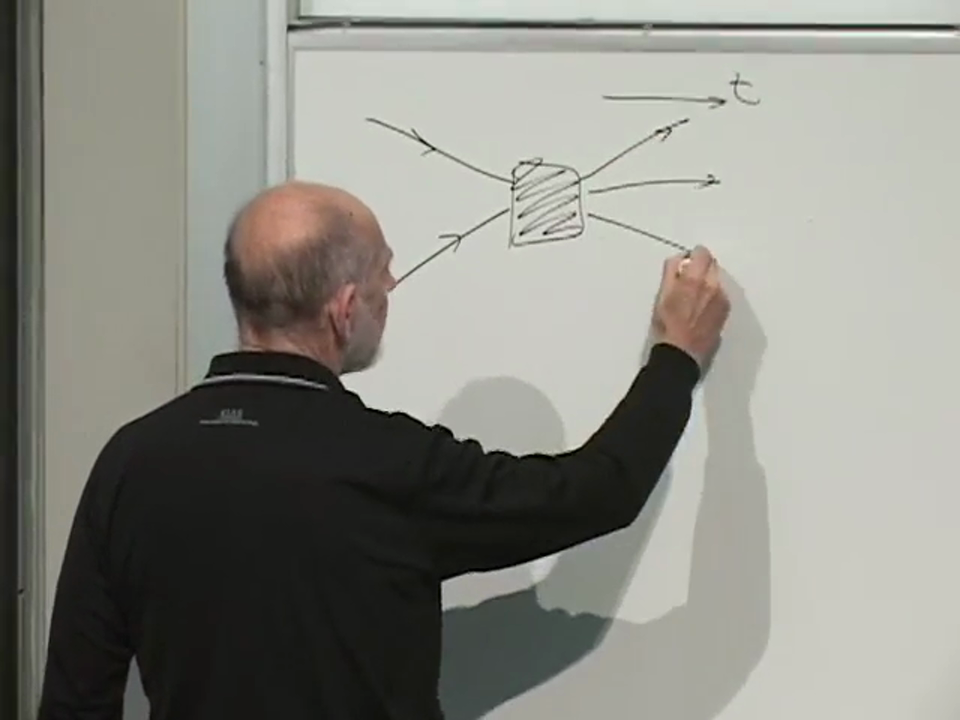
\includegraphics[width=0.72\textwidth]{lecture_06_figure_01.png}
  \caption{入射粒子が黒箱の相互作用領域に入り、出射粒子が出てくる。時間は水平に描かれている。}
  \lectureframe{00:02:35}
  \label{fig:l06-black-box}
\end{figure}

粒子はスピン、電荷、種類のラベルも持つ。まず運動学を明らかにするため、運動量以外のすべてを一時的に抑制しよう。

\section{四元運動量と全入射規約}

1つの粒子の四元運動量を
\begin{equation}
  k^\mu=(k^0,\mathbf k)=(E,\mathbf p).
\end{equation}
と書く。講義ではmostly-plus計量を用いるので、
\begin{equation}
  k^2\equiv \mathbf p^2-E^2.
\end{equation}
したがって相対論的分散関係は
\begin{equation}
  E^2-\mathbf p^2=m^2,
  \qquad
  k^2=-m^2.
  \label{eq:l06-mass-shell}
\end{equation}
である。空間運動量を変えるとエネルギーは変わるが、粒子を質量殻から外すことはない。

\begin{figure}[H]
  \centering
  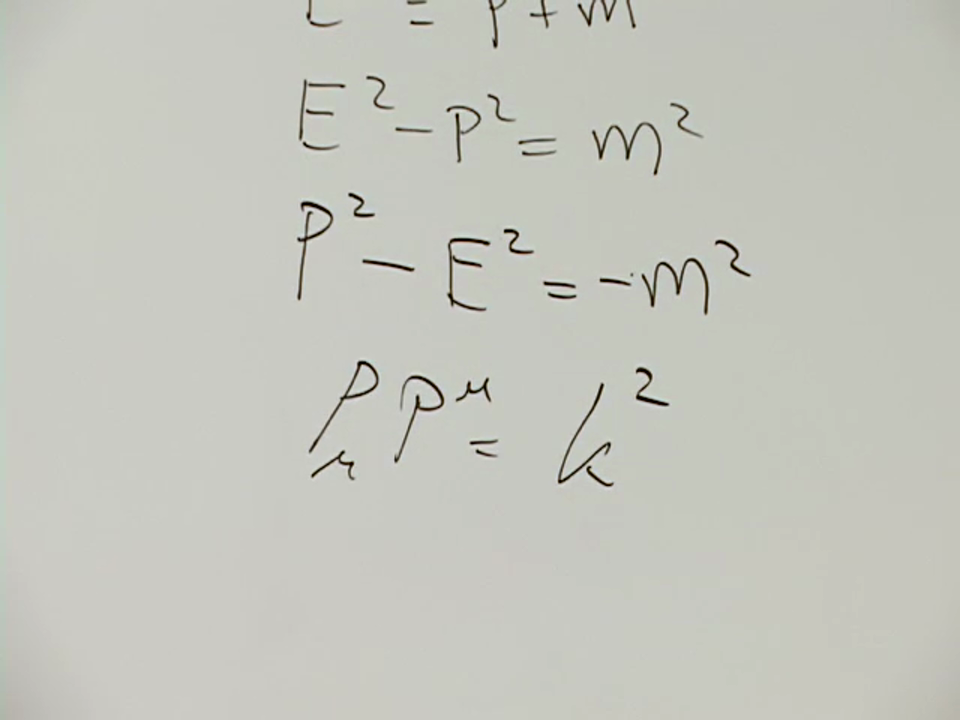
\includegraphics[width=0.66\textwidth]{lecture_06_figure_02.png}
  \caption{講義全体で用いられる計量規約における質量殻条件。}
  \lectureframe{00:05:56}
  \label{fig:l06-mass-shell}
\end{figure}

運動量\(k_1,k_2\)で入射する2個の粒子と、物理的運動量\(q_3,q_4\)で出ていく2個の粒子を考える。エネルギーと運動量の保存は1つの四元ベクトル方程式である。
\begin{equation}
  k_1+k_2=q_3+q_4.
  \label{eq:l06-physical-conservation}
\end{equation}
すべての外部線に進入運動量を割り当てると便利である。
\begin{equation}
  k_3\equiv-q_3,
  \qquad
  k_4\equiv-q_4.
\end{equation}
このとき
\begin{equation}
  k_1+k_2+k_3+k_4=0,
  \label{eq:l06-all-incoming}
\end{equation}
であり、各脚は\(k_i^2=-m_i^2\)を満たす。出ていく粒子が負のエネルギーをもつのはこの記帳法においてのみであり、それらの物理的エネルギーは正のままである。

\begin{figure}[H]
  \centering
  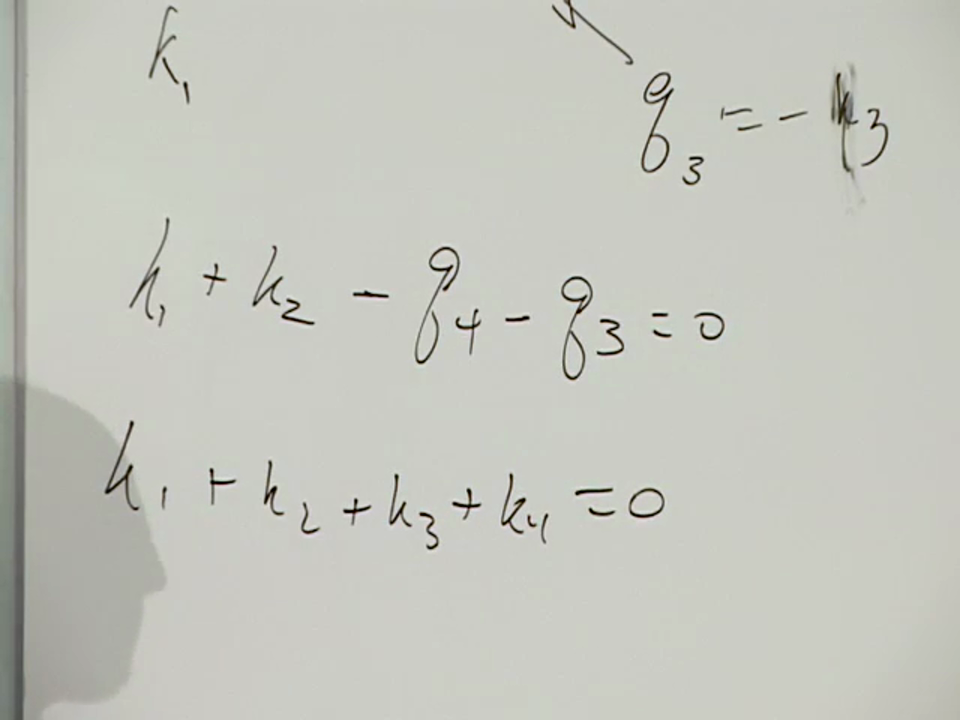
\includegraphics[width=0.68\textwidth]{lecture_06_figure_03.png}
  \caption{物理的な出射運動量は反転され、4つの外部運動量すべてを入射として対称に扱えるようにする。}
  \lectureframe{00:09:10}
  \label{fig:l06-all-incoming-board}
\end{figure}

一見すると振幅は16個の成分の関数\(\mathcal A(k_1,k_2,k_3,k_4)\)に見える。そのほとんどは冗長である。重心系に移り、入射運動量を選んだ軸へ回転し、簡単のため4つの粒子がすべて同じ質量を持つと仮定する。すると入射状態は1つの数、重心系エネルギーによって固定される。出射空間運動量は大きさが等しく逆向きで、入射対と同じ大きさでなければならない。残るのはその偏向角\(\theta\)だけである。したがってこの過程には2つの独立な運動学的変数がある。
\begin{equation}
  E_{\mathrm{cm}},
  \qquad
  \theta.
  \label{eq:l06-two-data}
\end{equation}

\section{マンデルスタム変数}

\eqref{eq:l06-two-data}における2つの物理量は、座標系を選ぶことなく表せるはずである。全入射規約で
\begin{equation}
  \begin{aligned}
    -s&=(k_1+k_2)^2,\\
    -t&=(k_1+k_3)^2,\\
    -u&=(k_1+k_4)^2.
  \end{aligned}
  \label{eq:l06-mandelstam}
\end{equation}
と定義する。重心系では\(k_1+k_2\)の空間部分が相殺するので、
\begin{equation}
  s=E_{\mathrm{cm}}^2.
  \label{eq:l06-s-energy}
\end{equation}

出射物理的運動量\(q_3=-k_3\)に対して、
\begin{equation}
  k_1+k_3=k_1-q_3
\end{equation}
は脚1から脚3へ移された運動量である。外部質量が等しく、入射空間運動量の大きさを\(p\)とすると、
\begin{equation}
  -t=2p^2(1-\cos\theta),
  \qquad
  -u=2p^2(1+\cos\theta).
  \label{eq:l06-tu-angle}
\end{equation}
したがって\(t\)と\(u\)は検出器が測定する角度情報を担う。

\begin{figure}[H]
  \centering
  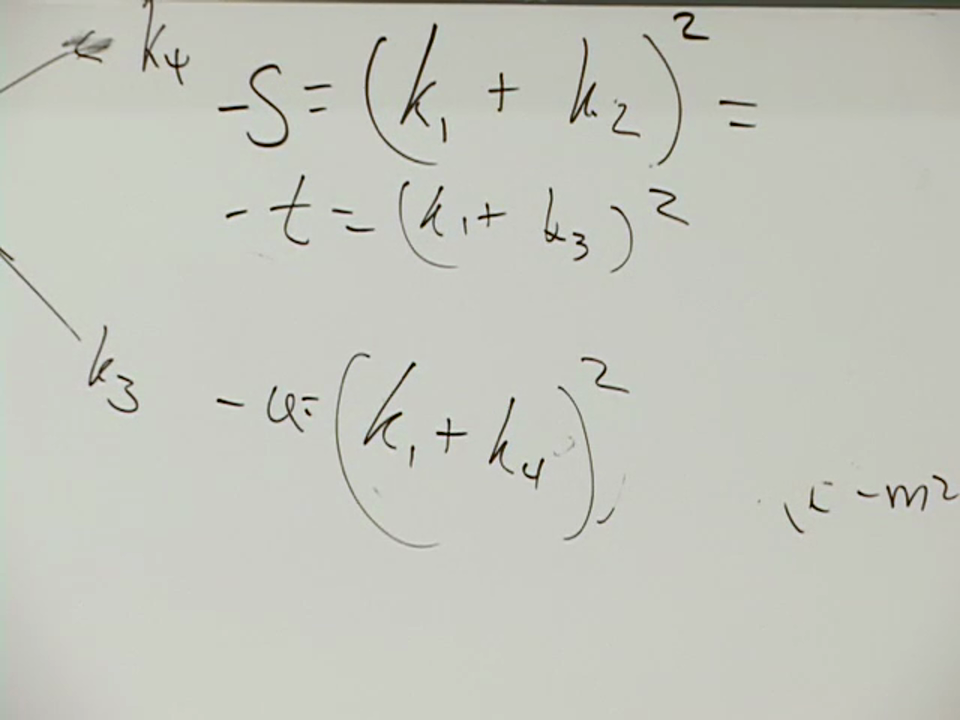
\includegraphics[width=0.74\textwidth]{lecture_06_figure_04.png}
  \caption{全入射規約における\(s,t,u\)の対称な定義。}
  \lectureframe{00:26:20}
  \label{fig:l06-stu-board}
\end{figure}

3つの記号は3つの独立なデータを意味するのではない。\eqref{eq:l06-all-incoming}を二乗し、\(k_i^2=-m^2\)を用いると、等しい質量に対して
\begin{equation}
  s+t+u=4m^2
  \label{eq:l06-stu-constraint}
\end{equation}
が得られる。\(s\)と\(t\)がわかれば、\(u\)は固定される。

\begin{classroomqa}
\audiencequestion{真空は、摩擦力のように、自由に運動する粒子を減速させることができるのだろうか？ \lecturetimestamp{00:27:17}}
\lecturerresponse{並進不変な真空では、それは起こらない。失われた運動量の行き先がどこにもないので、運動量保存則がそのような摩擦を禁じている。ある媒質や、特別な静止系を選び出す別の真空を想像することはできるが、それはここで用いている真空ではない。}
\end{classroomqa}

\begin{classroomqa}
\audiencequestion{なぜ2つの出射粒子は等しいエネルギーをもたなければならないのか？ \lecturetimestamp{00:27:54}}
\lecturerresponse{重心系では、それらの空間的運動量は大きさが等しく逆向きでなければならない。ここで議論している等質量の過程では、運動量の大きさが等しいことから、\(E^2=p^2+m^2\)を通じてエネルギーも等しくなる。もし出射粒子の質量が異なれば、この最後の結論は修正されなければならないだろう。}
\end{classroomqa}

\section{直接チャネルと交差チャネル}

単純な点粒子の図では、粒子1と2が質量\(M\)の中間粒子を形成し、それがその後3と4に崩壊する。分子の因子と極の処方を除けば、その特徴的な依存性は
\begin{equation}
  \mathcal A_s\sim\frac{g^2}{s-M^2}.
  \label{eq:l06-s-channel}
\end{equation}
である。これが直接過程、すなわち\(s\)チャネル過程である。連結の仕方を横向きにすると、2本の外線の間の交換、
\begin{equation}
  \mathcal A_t\sim\frac{g^2}{t-M^2},
  \label{eq:l06-t-channel}
\end{equation}
すなわち交差過程、\(t\)チャネル過程が得られる。第3の連結の仕方からは
\begin{equation}
  \mathcal A_u\sim\frac{g^2}{u-M^2}.
  \label{eq:l06-u-channel}
\end{equation}
が得られる。

\begin{figure}[H]
  \centering
  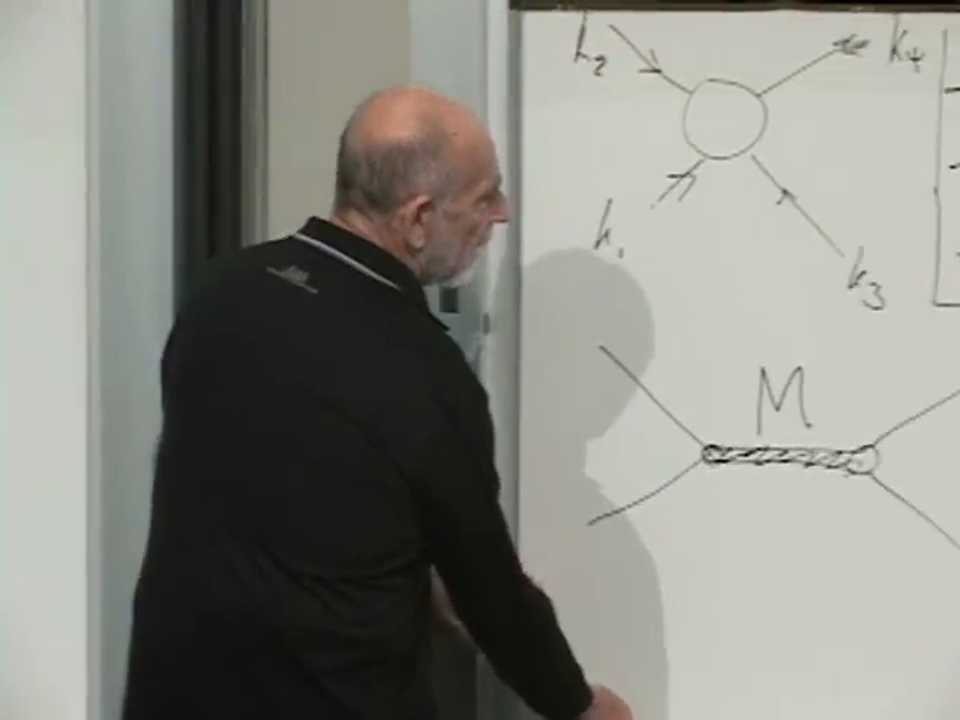
\includegraphics[width=0.72\textwidth]{lecture_06_figure_05.png}
  \caption{中間状態を通じた直接生成と、それに対応する極\(g^2/(s-M^2)\)。交差した連結の仕方は同じボード上で組み立てられつつある。}
  \lectureframe{00:30:50}
  \label{fig:l06-channel-board}
\end{figure}

この区別は物理的である。この粗いスカラー的な段階では、\eqref{eq:l06-s-channel}は衝突エネルギーに依存するが、角度には依存しない。複合状態は崩壊する前に入射方向を忘れてしまっているので、その崩壊は等方的である。交換振幅は運動量移行に依存し、したがって角度にも依存する。軽い交換粒子は小さな偏向を強く好む。スピンがあればさらに角度依存性が加わるだろうが、極の構造はすでに見えている。

\begin{classroomqa}
\audiencequestion{欠けている\(u\)チャネルは第3の項を生み出すのか？ \lecturetimestamp{00:34:47}}
\lecturerresponse{はい、粒子の同一性と結合がその連結の仕方を許すときはいつでもそうである。その場合には\(u=M^2\)に極をもつ項を含めることになる。\(s+t+u=4m^2\)であるから、これは新しい独立な運動学的変数ではないが、別個のチャネル図ではある。}
\end{classroomqa}

\section{1つの関数、2つのチャネル記述}

1つの極は中間子散乱の模型としては貧弱である。2つの中間子は、質量と角運動量の塔をもつ多数の共鳴状態を形成しうる。1960年代の最初の対応は、より多くの\(s\)チャネル極、より多くの\(t\)チャネル極、および許される\(u\)チャネル極を加えることであった。その後、はるかに経済的な関数が見出された。線形レッジェ軌跡とその切片が\(s\)および\(t\)に吸収されている講義の単位では、それは
\begin{equation}
  \mathcal A_{\mathrm V}(s,t)
  \propto
  \frac{\Gamma(-s)\Gamma(-t)}{\Gamma(-s-t)}.
  \label{eq:l06-veneziano}
\end{equation}
である。ガンマ関数は階乗を次のように延長する：
\begin{equation}
  \Gamma(n)=(n-1)!
\end{equation}
正の整数において。

\begin{figure}[H]
  \centering
  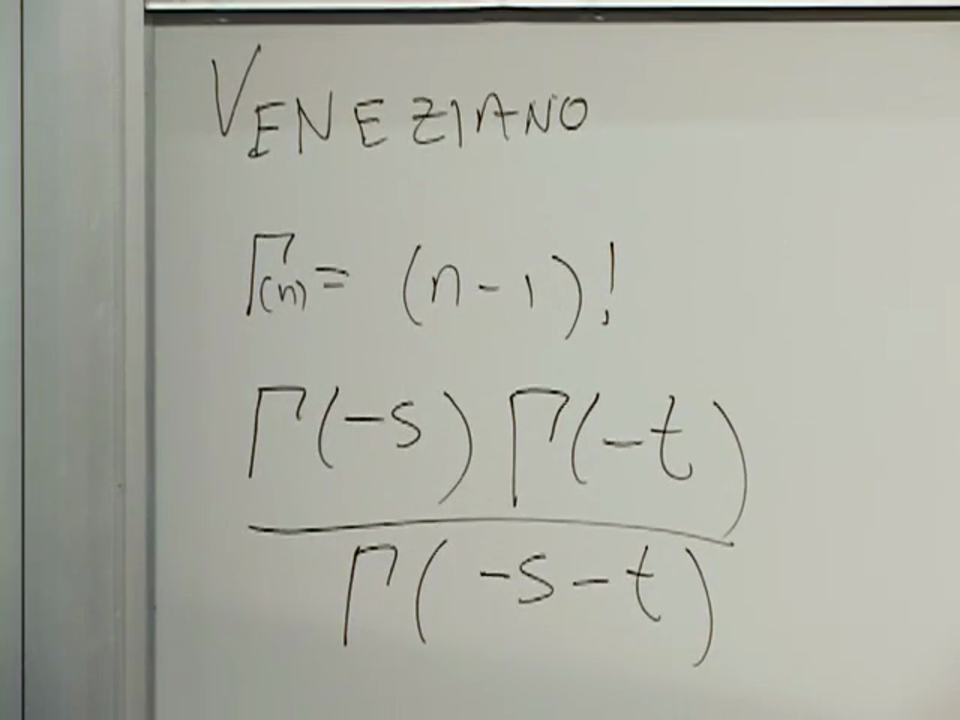
\includegraphics[width=0.68\textwidth]{lecture_06_figure_06.png}
  \caption{ガンマ関数の対称な比として書かれたヴェネツィアーノ振幅。}
  \lectureframe{00:42:25}
  \label{fig:l06-veneziano-board}
\end{figure}

\(\Gamma(-s)\)の極は、直接チャネル共鳴状態の無限の塔を再現する。しかし同じ表式は\(s\leftrightarrow
t\)の下で対称であるから、その\(\Gamma(-t)\)の極は交差チャネル展開を与える。これらは別々に加えられた2つの寄与ではない。1つの解析関数がどちらの記述も許容するのである。これが、直接チャネル共鳴状態と交差チャネル交換の間の双対性という古い考え方である。

\begin{classroomqa}
\audiencequestion{1つの振幅が、両方のチャネル和を加え合わせることなく、どのようにして両方を含むことができるのか？ \lecturetimestamp{00:43:32}}
\lecturerresponse{まさにそこが驚きである。関数をその\(s\)チャネル極の近くで展開すると、直接共鳴状態として整理される。その\(t\)チャネル極の近くで展開すると、同じ関数が交換として整理される。なぜこれら2つの読み方が同じであるのかを説明するには微視的模型が必要であり、その模型が相互作用する弦である。}
\end{classroomqa}

\section{開弦が掃き出す帯}

開弦を次のようにパラメータ付けする：
\begin{equation}
  0\leq\sigma\leq\pi.
\end{equation}
ラベル\(\sigma\)は時空の位置ではない。埋め込み\(X^\mu(\sigma,\tau)\)は、そのラベル付けされた点が時空のどこにあるかを教え、一方\(\tau\)は発展を測る。点粒子は世界線を掃き出すが、運動する弦は2次元の世界面を掃き出す。自由理論では、各埋め込み座標は次を満たす：
\begin{equation}
  \frac{\partial^2X^\mu}{\partial\tau^2}
  -
  \frac{\partial^2X^\mu}{\partial\sigma^2}
  =0.
  \label{eq:l06-wave-equation}
\end{equation}

\begin{figure}[H]
  \centering
  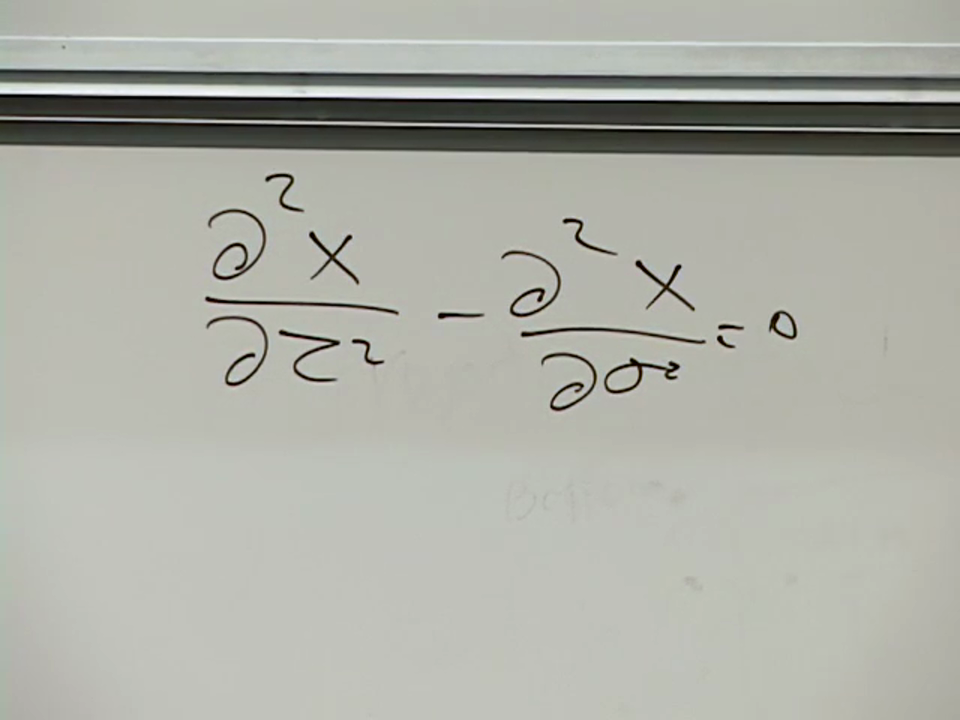
\includegraphics[width=0.70\textwidth]{lecture_06_figure_07.png}
  \caption{世界面の帯上で各自由弦座標を支配する波動方程式。}
  \lectureframe{00:49:10}
  \label{fig:l06-wave-equation-board}
\end{figure}

散乱の構成には、連続極限を早急に取らない方が有用である。各弦を\(n\)個の質点がばねで結ばれたものに置き換える。世界面は近接する世界線の密な集まりとなり、その基準モードは通常の調和振動子である。二つの入射鎖は端点で接触しうる。その事象で新しいばねがそれらを結び、それらは時間\(\tau\)の間、一つのより長い鎖として発展し、後にばねが切れて二つの出射鎖が現れる。

\begin{figure}[H]
  \centering
  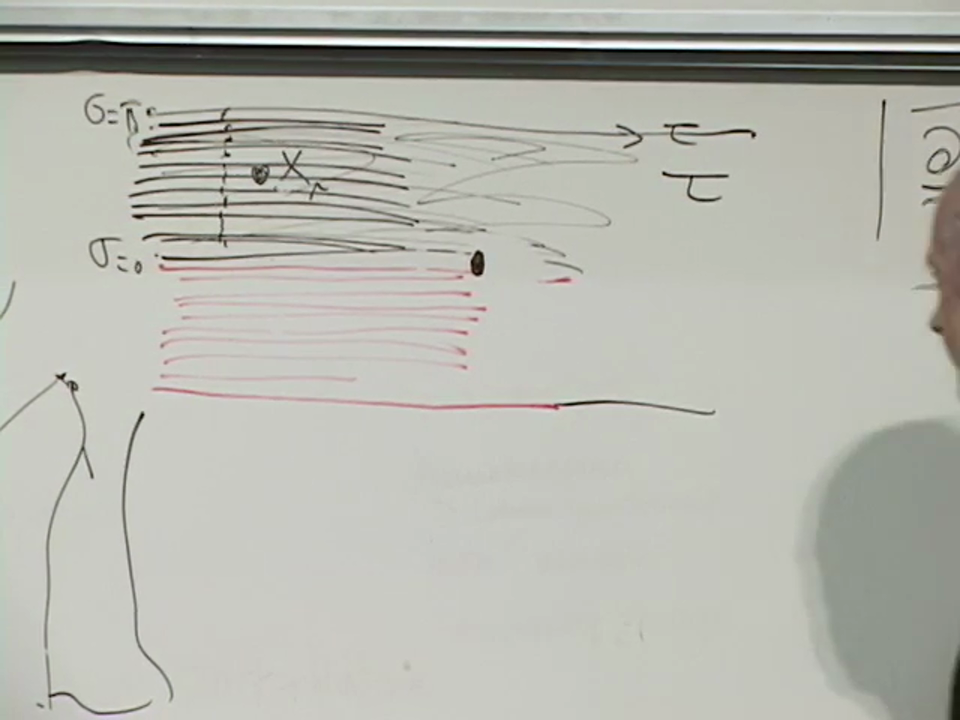
\includegraphics[width=0.72\textwidth]{lecture_06_figure_08.png}
  \medskip

  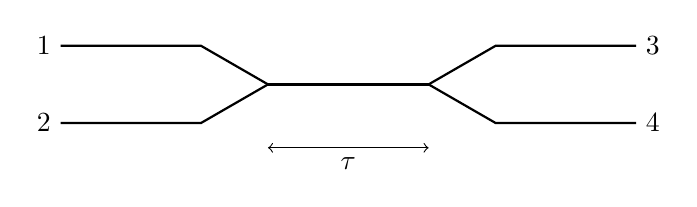
\begin{tikzpicture}[x=0.85cm,y=0.70cm]
    \draw[thick] (0,2.2) -- (2.1,2.2) -- (3.1,1.5);
    \draw[thick] (0,0.8) -- (2.1,0.8) -- (3.1,1.5);
    \draw[thick] (3.1,1.5) -- (5.5,1.5);
    \draw[thick] (5.5,1.5) -- (6.5,2.2) -- (8.6,2.2);
    \draw[thick] (5.5,1.5) -- (6.5,0.8) -- (8.6,0.8);
    \draw[<->] (3.1,0.35) -- node[below] {\(\tau\)} (5.5,0.35);
    \node[left] at (0,2.2) {1};
    \node[left] at (0,0.8) {2};
    \node[right] at (8.6,2.2) {3};
    \node[right] at (8.6,0.8) {4};
  \end{tikzpicture}
  \caption{二つの離散化された開弦が接触し、時間\(\tau\)の間、一つの中間弦を形成して、分裂する。元のフレームはばねと世界線の構成を保ち、模式図はその連結性を分離して示す。}
  \lectureframe{00:51:25}
  \label{fig:l06-string-joining}
\end{figure}

二つの弦はパラメータ空間においてのみ隣接して描かれている。それらの時空位置は、端点座標が実際に一致するまでは隣接している必要はない。再パラメータ化の自由度により、結合と分裂の事象を図上の都合のよい位置に置くことができる。この幾何学的自由度は次の講義で共形対称性となる。

\section{振動子計算のスローモーション}

第一の鎖の座標を\(x_1,\ldots,x_n\)、第二の鎖の座標を\(x_{n+1},\ldots,x_{2n}\)とする。それらの重心座標は
\begin{equation}
  X_{\mathrm{cm}}^{(1)}
  =\frac1n\sum_{a=1}^{n}x_a,
  \qquad
  X_{\mathrm{cm}}^{(2)}
  =\frac1n\sum_{a=n+1}^{2n}x_a.
  \label{eq:l06-chain-centers}
\end{equation}
である。確定した運動量\(k_1\)をもつ鎖は、内部振動子の基底状態に重心平面波を掛けたものである：
\begin{align}
  \Psi_1
  &=
  e^{ik_1\cdot X_{\mathrm{cm}}^{(1)}}
  \psi_0(x_1,\ldots,x_n),
  \\
  \Psi_2
  &=
  e^{ik_2\cdot X_{\mathrm{cm}}^{(2)}}
  \psi_0(x_{n+1},\ldots,x_{2n}).
  \label{eq:l06-two-wavefunctions}
\end{align}
因子\(\psi_0\)は相対座標に依存し、鎖全体の共通並進には依存しない。入射弦は初め別々の量子系であるから、
\begin{equation}
  \Psi_{\mathrm{in}}=\Psi_1\Psi_2.
  \label{eq:l06-product-state}
\end{equation}

\begin{figure}[H]
  \centering
  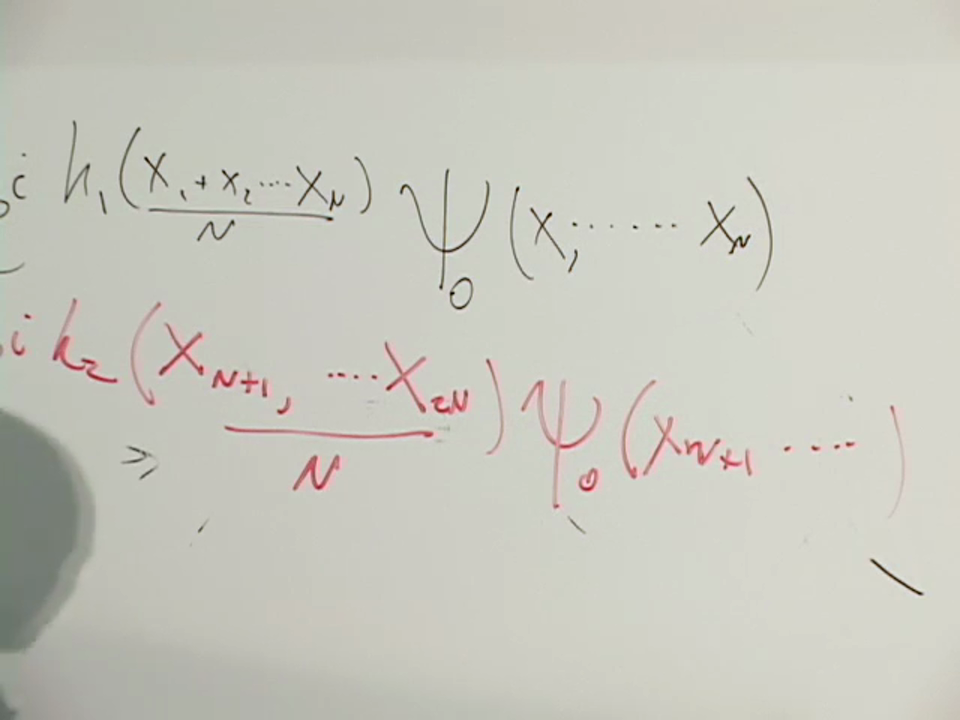
\includegraphics[width=0.76\textwidth]{lecture_06_figure_09.png}
  \caption{二つの運動量平面波とそれらの内部振動子基底状態因子を、別々の色で書いたもの。}
  \lectureframe{00:58:05}
  \label{fig:l06-wavefunctions-board}
\end{figure}

結合は、二つの端点座標が一致するこの波動関数の部分を選び出す：
\begin{equation}
  x_n=x_{n+1}.
  \label{eq:l06-endpoint-contact}
\end{equation}
その瞬間、他の座標は変わらない。選ばれた状態は次に、一つのより長い鎖のハミルトニアン\(H_{\mathrm{joined}}\)で発展させられる：
\begin{equation}
  \Psi(\tau)
  =
  e^{-iH_{\mathrm{joined}}\tau}\Psi(0).
  \label{eq:l06-time-evolution}
\end{equation}
最後に、運動量\(q_3,q_4\)をもつ出射弦状態の積との重なりを取る。

\begin{figure}[H]
  \centering
  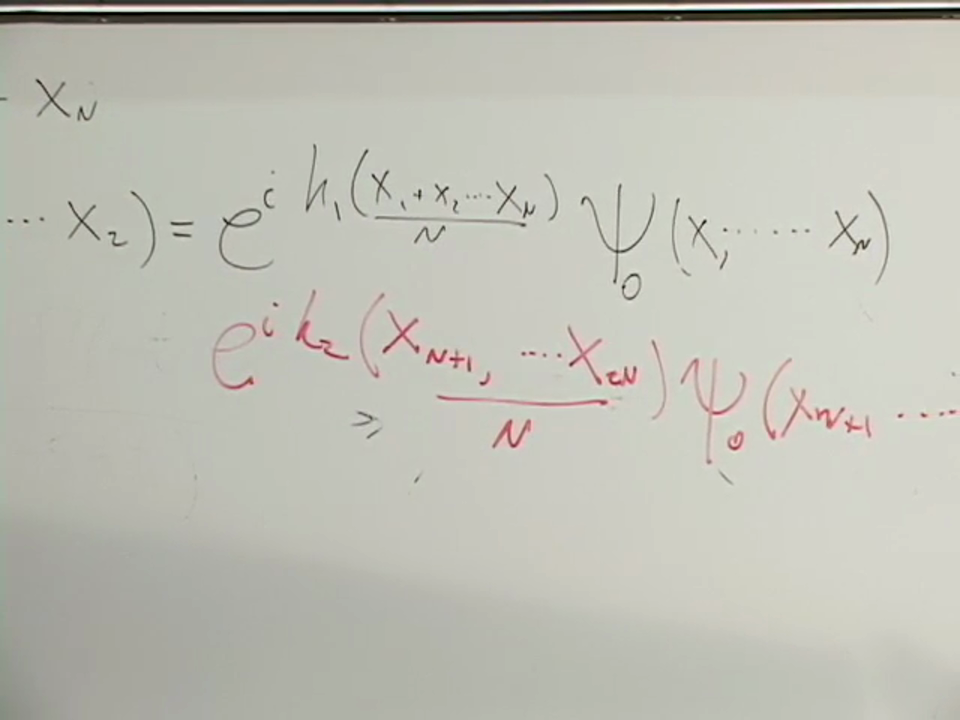
\includegraphics[width=0.76\textwidth]{lecture_06_figure_10.png}
  \caption{端点の一致を課す直前の二鎖波動関数。}
  \lectureframe{00:58:55}
  \label{fig:l06-endpoint-board}
\end{figure}

計算は長いが不可解ではない。すべての内部座標は振動子モードに分解できるので、結合の重なり、時間発展、最終的な射影はガウス的振動子代数に帰着する。未確定のまま残るのは、結合した弦の寿命\(\tau\)である。

\begin{classroomqa}
\audiencequestion{黒と赤の波動関数は加えられるのか、掛けられるのか。\lecturetimestamp{01:02:26}}
\lecturerresponse{掛けられる。二つの独立な系のテンソル積状態は、座標基底ではそれらの波動関数の積で表される。加えることは選択肢の重ね合わせを記述することになり、二つの入射弦が同時に存在することにはならない。}
\end{classroomqa}

\begin{classroomqa}
\audiencequestion{なぜ中間時間\(\tau\)について積分するのか。\lecturetimestamp{01:04:04}}
\lecturerresponse{結合した弦には確定した寿命が割り当てられていない。ファインマンの規則は、すべての許された履歴にわたって振幅を和することである。この記述では、残る連続的な履歴パラメータは結合と分裂の間の時間であるから、和は\(0\leq\tau<\infty\)にわたる積分となる。}
\end{classroomqa}

\section{伝播時間からベータ関数へ}

振動子の重なりを評価した後、結果は次のように整理できる：
\begin{equation}
  \mathcal A(s,t)
  \propto
  \int_0^\infty d\tau\,
  e^{\tau(s+1)}
  \bigl(1-e^{-\tau}\bigr)^{-t-1}
  e^{-\tau}.
  \label{eq:l06-tau-integral}
\end{equation}
最後の\(e^{-\tau}\)は、次の段階で必要となるヤコビアンであるため、見える形で保たれている。等価に、最初と最後の指数関数は結合して\(e^{s\tau}\)となる。

\begin{figure}[H]
  \centering
  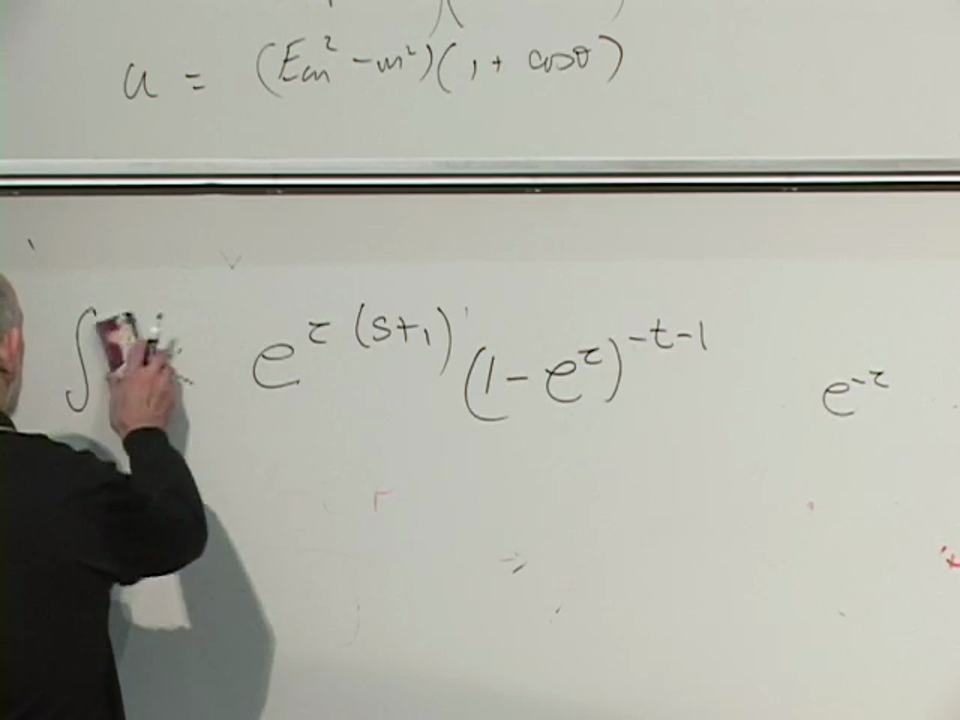
\includegraphics[width=0.76\textwidth]{lecture_06_figure_11.png}
  \caption{振動子計算後の伝播時間被積分関数。分離した\(e^{-\tau}\)因子が変数変換のヤコビアンを与える。}
  \lectureframe{01:06:45}
  \label{fig:l06-tau-integral-board}
\end{figure}

ここで
\begin{equation}
  z=e^{-\tau},
  \qquad
  dz=-e^{-\tau}\,d\tau.
  \label{eq:l06-z-substitution}
\end{equation}
と置く。\(\tau\)が\(0\)から\(\infty\)まで動くとき、\(z\)は\(1\)から\(0\)まで動く。負号は積分限界を逆転させ、
\begin{equation}
  \mathcal A(s,t)
  \propto
  \int_0^1
  z^{-s-1}(1-z)^{-t-1}\,dz.
  \label{eq:l06-beta-integral}
\end{equation}
を与える。

\begin{figure}[H]
  \centering
  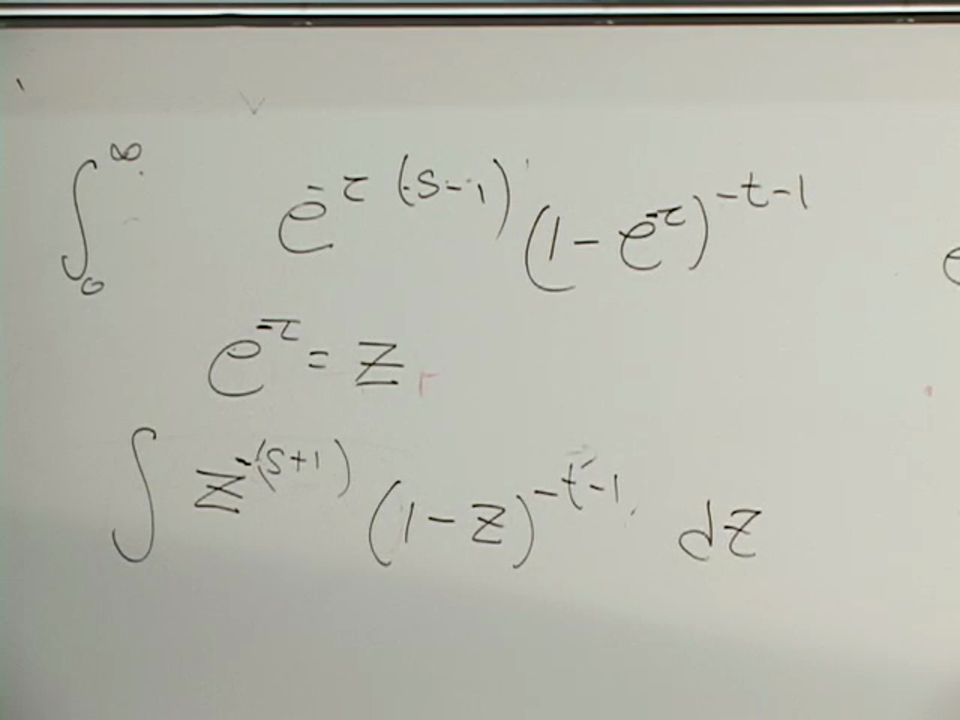
\includegraphics[width=0.74\textwidth]{lecture_06_figure_12.png}
  \caption{置換\(z=e^{-\tau}\)がオイラーベータ積分を露わにする。}
  \lectureframe{01:08:49}
  \label{fig:l06-beta-integral-board}
\end{figure}

この積分は、その端点が収束する場所では直接定義され、それ以外では解析接続によって定義される。これはオイラーベータ関数である：
\begin{equation}
  B(-s,-t)
  =
  \frac{\Gamma(-s)\Gamma(-t)}{\Gamma(-s-t)}.
  \label{eq:l06-beta-gamma}
\end{equation}

\begin{figure}[H]
  \centering
  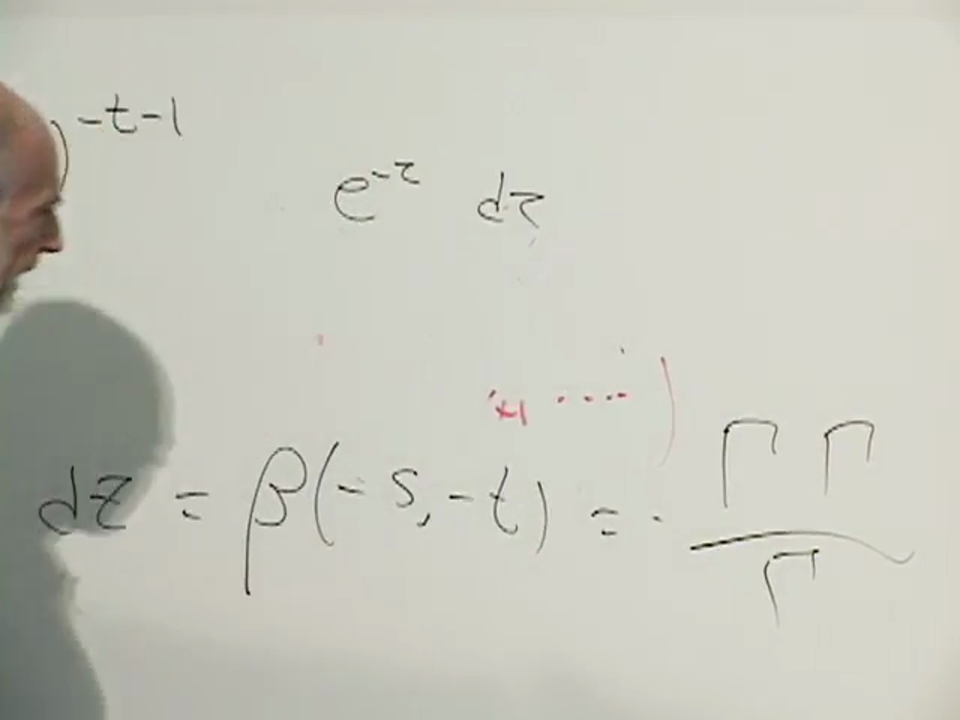
\includegraphics[width=0.72\textwidth]{lecture_06_figure_13.png}
  \caption{黒板は変換された積分を\(B(-s,-t)\)と同定し、そのガンマ関数の形を復元し始める。}
  \lectureframe{01:12:24}
  \label{fig:l06-beta-gamma-board}
\end{figure}

チャネル対称性は今や初等的である。\(z\mapsto1-z\) の下で、
\begin{equation}
  \int_0^1 z^{-s-1}(1-z)^{-t-1}\,dz
  =
  \int_0^1 z^{-t-1}(1-z)^{-s-1}\,dz.
\end{equation}
したがって \(\mathcal A(s,t)=\mathcal A(t,s)\) である。二つの弦が結合し、後に分裂する過程として構成された過程は、自動的に交差した記述も含んでいる。
\editorialnote{講義ではベータ関数の引数におけるレッジェ傾きと切片を省略している。標準的な記法では \(s,t\) を対応する線形軌跡 \(\alpha(s),\alpha(t)\) に置き換える。双対性と変数変換の議論は変わらない。}

\begin{classroomqa}
\audiencequestion{ガンマ関数の比は組合せ論における階乗の式に似ている。直接的な物理的計数の解釈はあるのだろうか？ \lecturetimestamp{01:13:22}}
\lecturerresponse{整数引数ではベータ関数は \(n!\,m!/(n+m)!\) のような比に関係するが、ここで組合せ論的な機構を主張しているわけではない。同じ特殊関数が世界面積分からたまたま現れるのであり、この類似が振幅を見出した経路であったわけではない。}
\end{classroomqa}

一つの世界面が両方のチャネルで読める、まだ隠された理由は共形対称性である。それは振幅を変えずに面をタフィーのように引き伸ばすことを許し、長い直接チャネルの伝播領域を交差チャネルの交換描像へと変える。その幾何学的説明は次の講義に延期される。

\section{散乱テストが確立したこと}
\enlargethispage{3\baselineskip}
\begingroup
\setlength{\medskipamount}{3pt plus 1pt minus 1pt}

離散的な結合描像は、最後の一群の質問を促した。

\begin{classroomqa}
\audiencequestion{\(n\) 個の構成要素からなる二つの鎖が端点で結合するなら、結果は \(2n-1\) であり、それはフェルミオン・パリティを変えうるだろうか？ \lecturetimestamp{01:16:16}}
\lecturerresponse{ハドロン的端点描像では、接触する端点対は対消滅する粒子・反粒子対と見なせるので、数は一つではなく二つ減る。連続極限では \(2n\) と \(2n-2\) の有限な差は重要でないが、フェルミオン・パリティの保存は重要である。格子構成要素は連続弦のための単なる正則化であり、文字通りの基本的なビーズではない。}
\end{classroomqa}

\begin{classroomqa}
\audiencequestion{後の議論は超弦の完全な数学へと続くだろうか？ \lecturetimestamp{01:18:05}}
\lecturerresponse{選ばれた帰結のみが用いられる。当面の道筋は世界面対称性とコンパクト化を通り、続いて 1990 年代半ばに発展した別の出発点、すなわちM理論である。その目的は、そうでなければ複雑ないくつかの特徴が透明になる視点から同じ物理に到達することである。}
\end{classroomqa}

\begin{classroomqa}
\audiencequestion{この結合規則はメソン衝突からの手がかりにすぎなかったのか？ \lecturetimestamp{01:20:02}}
\lecturerresponse{メソン散乱が歴史的な手がかりを与えたが、この規則は開弦に対して一般的である。同じトポロジーが開弦光子や他の開弦状態の衝突を記述する。二つの閉弦は類似の構成で結合し分裂し、中間領域には閉弦が存在する。}
\end{classroomqa}

\begin{classroomqa}
\audiencequestion{この計算は弦の状態がフェルミオンである場合にのみ適用されるのか？ \lecturetimestamp{01:20:56}}
\lecturerresponse{いいえ。元のヴェネツィアーノの計算はボソン的開弦に属する。超弦は追加のフェルミオン的自由度を必要とし、被積分関数の詳細を変更するが、結合、伝播、射影、世界面双対性の論理は密接に類似したままである。}
\end{classroomqa}

振動子スペクトルにスピン1またはスピン2の状態を見出すことは示唆的であったが、決定的ではなかった。それらの散乱振幅がより強いテストを与えた。光子振幅は電荷保存とゲージ不変性に関連する恒等式を満たし、重力子振幅は質量ゼロのスピン2場に対応する制約を満たす。弦の状態は、質量のある状態および質量のない状態との相互作用、および互いの相互作用においてこれらのテストに合格した。だからこそ光子と重力子というラベルは、偏極の計数のみに基づく推測ではなく、物理的同定となったのである。
\editorialnote{現代的な言葉では、これらのテストは非物理的偏極の脱結合、ゲージ・ウォード恒等式、および質量ゼロのスピン2状態の普遍的低エネルギー結合に符号化されている。}

\begin{classroomqa}
\audiencequestion{弦の記述において電荷そのものはどこから来るのか？ \lecturetimestamp{01:24:03}}
\lecturerresponse{その問いは講義の終わりに未解決のまま残される。その答えには弦理論の内部構造と端点構造が必要であり、それらはまだ導入されていないので、この散乱の導出ではなく、続く議論に属する。}
\end{classroomqa}
\endgroup
